\section{Einführung}

Fundamental in den Wirtschaftswissenschaften ist die von Frank H.Knight eingeführte Unterscheidung zwischen Risiko und Unsicherheit. Risiko wird von Knight als quantifizierbare 
Unsicherheit definiert, also besipielsweise eine Situatuin in welcher jedem möglichen Ausgang eine Wahrscheinlichkeit zugeschrieben werden kann. Klassische Beispiele hierzu sind 
Versicherungen oder Glücksspiel im Casino, wo ein Gewinn zwar unsicher ist, man aber weiß, dass die Kugel mit einer Wahrscheinlichkeit von $p = 1/37$ auf einem spezifischen Feld 
landen wird.

Die von Knight definierte Unsicherheit hingegen, in seinen Worten "echte Unsicherheit", bezieht sich auf Situationen, in denen man den Ausgängen eben keine definitive Wahrscheinlichkeit zuordnen kann.
Dies ist beispielsweise der Fall, wenn keine historischen Daten vorhanden sind, an denen man die Wahrscheinlichkeiten ableiten könnten. \cite{Knight1921} Ein reales Beispiel dafür wäre der Marktstart eines neuartigen, innovativen Produktes, 
welches noch keine Vergleichbaren Wettbewerber hatte. Netflix's Streaming Service käme in den Kopf. 

In der heutigen Welt, welche von Innovation und Schnellebigkeit geprägt ist, ist das Verständnis von Risiko und Unsicherheit von besonderer Bedeutung. Unternehmer müssen andauernd Entscheidungen treffen, welche umfangreiche Konsequenzen haben könnten. 
Die Fähigkeit Unsicherheiten richtig einzuschätzen, darstellen und eventuell auch nutzen zu können, kann dabei den Unterschied zwischen Erfolg und Misserfolg ausmachen. 

Wenn man den Punkt Darstellung von Unsicherheit heranzieht und in die Domäne der Datenvisualisierung eintaucht, trifft man auf viele ähnliche jedoch auch zahlreiche unterschiedliche Definitionen dieser 
im Vergleich zu Knight. 

Haber und McNabb \cite{Haber1990} beschreiben einen Art Visualisierungs-Pipeline, welche in vielen Papern der Unsicherheitsvisualisierung aufgegriffen wird, unter anderem in einem Standardpaper von Pang et al. \cite{Pang1997}.
Bei dieser wird in jedem Schritt, von der Datenbeschaffung bis zur entgültigen Visualisierung, ein Teil Unsicherheit eingeschleußt oder ist inherent vorhanden, weshalb diese Berücksichtigt werden muss. Im Grunde läuft sie wie folgt ab:

\begin{enumerate}
    \item \textbf{Datenbeschaffung}:
    In dieser Phase ist Unsicherheit immer vorhanden, sei es durch Messfehler oder -ungenauigkeiten, die Beschaffung der Daten durch statistische Modelle oder unvollständige Daten, eine Messung kann nie zu 100\% genau sein.
    
    \item \textbf{Datenvorverarbeitung}:
    Die beschafften Daten müssen in einem nachfolgenden Schritt aufbereitet werden, in welchem durch Interpolation von fehlenden Daten, ungenaue Transformationen oder Annahmen weitere Unsicherheit einfließen kann.
    
    \item \textbf{Datenverarbeitung und -analyse}:
    Diese Daten werden zur Visualisierung auf ein oder mehrere geometrische Objekte gemappt. Dies stellt durch die verwendeten Algorithmen und Modelle eine neue Quelle von Unsicherheit dar.
    
    \item \textbf{Visualisierung}:
    Schließlich werden die Daten visualisiert. Hier können Unsicherheiten durch die Wahl der Visualisierungstechniken und Darstellungsparameter wie Farbskalen und Fehlerbalken beeinflusst werden.
\end{enumerate}

Man erkennt viele verschieden Arten von Unsicherheit in dieser Pipeline. Seien es Messfehler oder falsche Annahmen. Es wird sich jedoch hauptsächlich auf Finanzprognosen bezogen, weshalb es hier um die in der nächsten Sektion beschriebenen Arten von Unsicherheit geht.


\subsection{Die Bedeutung von Unsicherheit in Finanzmärkten}
Eine weiter Ansichtsweise aus Knights Paper war ausserdem, dass ein Unternehmer nur wirtschaftlich erfolgreich sein kann, wenn dieser Unsicherheiten auf sich nimmt, da andernfalls jeder Wettbewerber die gleichen, 
korrekten Informationen hätte und somit kein Vorteil erarbeitet werden kann. Wird diese aufzunehmende Unsicherheit aber im Entscheidungsprozess falsch oder unzureichend dargestellt, kann dies fatale Folgen nach sich ziehen.

Man stelle sich beispielsweise die Prognose eines Aktienkurses anhand eines Monte-Carlo-Modells vor. Sollte ein Investor auf Basis dieser Prognose eine Entscheidung treffen, ist er einerseits mit der direkten quantitativen 
Unsicherheit der Vorhersage konfrontiert, also mit der Wahrscheinlichkeit, dass genau der gewählte Zweig der Simulation zutrifft. Andererseits gibt es die indirekte qualitative Unsicherheit: 
Hat der Ersteller korrekt historische Daten verwendet? \cite{Padilla2021} Auf welcher Basis von Zufall wurde die Prognose erstellt – Volatilität oder fundierte ökonomische Kennzahlen des Unternehmens? 
Es gil, diese Unsicherheiten so gut wie möglich darzustellen, um den Investor bei seiner Entscheidungsfindung zu unterstützen und keine Trugschlüsse zuzulassen.


\subsection{Ziele der Arbeit}
Deshalb wird in dieser Arbeit untersucht, wie sich die Visualisierung von Unsicherheiten und Risiken auf Entscheidungsträger auswirkt, 
wie Techniken angewandt werden können, um die Kommunikation von Informationen "sicherer" zu machen und zu verbessern. Dies geschieht im Rahmen der Finanzwelt.

Im folgenden Kapitel werden Grundlagen zur Entscheidungsfindung von Menschen und Techniken der Visualisierung von Unsicherheiten beleuchtet.


\section{Theorien zur Entscheidungsfindung unter Unsicherheit}
Es werden Theorien zur Entscheidungsfindung unter Unsicherheit näher beleuchtet, welche laut Padilla et al. \cite{VisualizationPsychology2023}  berücksichtigt werden müssen, um Visualisierungstechniken auf Basis ihrer Rolle in Entscheidungsfindungen unter Unsicherheit bewerten zu können. Diese werden in Sektion 3 wieder aufgegriffen, um den Effekt unterschiedlicher Visualisierungsmethoden auf die Entscheidungsfindung zu erklären.

\subsection{Erwartungsnutzentheorie}

Die Erwartungsnutzentheorie (EUT) ist ein grundlegendes Modell in der Entscheidungstheorie das beschreibt, wie rationale Akteure Entscheidungen unter Unsicherheit treffen sollten. Entwickelt von John von Neumann und Oskar Morgenstern, basiert die EUT auf der Annahme, dass Akteure bei der Wahl zwischen unsicheren Alternativen die Option bevorzugen, welche den höchsten erwarteten Nutzen bietet. Dieser erwartete Nutzen eines Ergebnisses wird dabei als das Produkt aus der Wahrscheinlichkeit des Ergebnisses und dem subjektiven Nutzen dieses berechnet.

Die mathematische Darstellung der Erwartungsnutzentheorie geht wie folgt:

\begin{equation}
EU = \sum_{i=1}^{n} p_i \cdot u(x_i)
\end{equation}

Dabei ist \( EU \) der erwartete Nutzen, \( p_i \) die Wahrscheinlichkeit des Ergebnisses \( x_i \) und \( u(x_i) \) der Nutzen des Ergebnisses \( x_i \).

Die EUT geht davon aus, dass Akteure gleichbleibende Präferenzen haben und immer die Alternative mit dem höchsten erwarteten Nutzen wählen \cite{vonNeumann1944}. Diese Theorie hat viele Anwendungen in der Finanzwelt, beispielsweise bei der Analyse von Investitionen und Risiken.

\subsection{Dual-Process-Theorie}

Die Dual-Process-Theorie beschreibt, wie Menschen zwei verschiedene Arten von Denkprozessen nutzen, um Entscheidungen zu treffen: intuitives (Type 1) und analytisches (Type 2) Denken. Die Grundlagen für diese Theorie wurden von Psychologen wie Daniel Kahneman und Keith Stanovich über Jahre entwickelt und heben hervor, dass Menschen je nach Situation und Komplexität der Aufgabe zwischen diesen beiden Denkmodi wechseln \cite{Tversky74}.

\begin{itemize}
    \item \textbf{Type 1 Prozesse}: Diese sind schnell, automatisch und erfordern wenig kognitive Anstrengung. Sie basieren auf Intuition, die oft aus Erfahrungen und erlernten Mustern hervorkommen. Type 1 Prozesse sind nützlich in routinemäßigen und vertrauten Situationen, können jedoch zu systematischen Fehlern und Trugschlüssen führen.
    \item \textbf{Type 2 Prozesse}: Diese sind langsam, bewusst und erfordern einiges an kognitiver Anstrengung. Sie basieren auf logischem Denken und systematischer Analyse. Type 2 Prozesse kommen zum Einsatz, wenn komplexe und neue Situationen eine tiefgehende Bewertung erfordern.
\end{itemize}

Die Dual-Process-Theorie erklärt, warum Menschen in vielen Situationen intuitive Entscheidungen treffen, die schnell und effizient sind, aber eben auch öfter zu suboptimalen Ergebnissen führen. Sie betont auch wie wichtig es ist, analytisches Denken zu fördern, insbesondere bei komplexen und wichtigen Entscheidungen, bei denen Fehler schwere Konsequenzen haben können.

\subsection{Vergleich der Theorien}

Die Erwartungsnutzentheorie und die Dual-Process-Theorie bieten unterschiedliche Perspektiven auf die Entscheidungsfindung unter Unsicherheit. Während die EUT ein Modell ist, das beschreibt wie Entscheidungen getroffen werden sollten, bietet die Dual-Process-Theorie ein beschreibendes Modell, das erklärt, wie Entscheidungen tatsächlich getroffen werden. Die EUT geht von rationalen und gleichbleibende Präferenzen aus, wohingegen die Dual-Process-Theorie die Rolle von Intuition betont, die zu systematischen Fehlern führen kann.

\section{Unsicherheitsvisualisierung zur Entscheidungsstützung}

Um die Bedeutung der Visualisierung von Unsicherheiten auf die Entscheidungsfindung besser zu verstehen, wird eine Fallstudie beleuchtet, welche genau das untersucht hat. Anschließend werden die beiden daraus resultierenden, erfolgversprechendsten Visualisierungsmethoden näher betrachtet.

\subsection{Fallstudie Fantasy Football}

In der Fallstudie von Kale et al. \cite{Kale2021} wurde untersucht, wie verschiedene Unsicherheitsvisualisierungen die Entscheidungsfindung beeinflussen können. Die Teilnehmer der Studie nahmen an einem fiktiven Fantasy-Football-Spiel teil, dessen Ziel es war, einen 3,7 Mio. Dollar Wettbewerb zu gewinnen. In diesem mussten Entscheidungen darüber getroffen werden, ob sie für Kosten von 1 Mio. Dollar einen neuen Spieler zu ihrem Team hinzufügen sollten oder nicht. Die Visualisierungen zeigten, wie viele Punkte sie ohne Hinzufügen des Spielers beziehungsweise nach Hinzufügen erzielen würden. 

Die Studie testete verschiedene Visualisierungsdesigns, darunter 95\%-Intervallbereiche, hypothetische Ergebnisszenarien, Dichteplots und Quantile Dotplots, jede mit und ohne Darstellung der Mittelwerte. Es wurde untersucht, anhand welcher Visualisierung am besten abgeschätzt wurde, ob es sinnvoll wäre, den neuen Spieler hinzuzufügen, um den höchsten monetären Gewinn (3,7 Mio. Dollar falls Gewinn ohne, 2,7 Mio. Dollar falls Gewinn mit Hinzufügen eines neuen Spielers) zu erzielen.

Die Ergebnisse der Studie zeigten, dass Quantile Dotplots die genaueste Abschätzung der Auswirkung und die besten Entscheidungen förderten, insbesondere bei geringer Varianz. Diese Methode half den Nutzern, die Unsicherheit intuitiver zu verstehen und bessere Entscheidungen zu treffen, indem sie Wahrscheinlichkeiten und Verteilungen klar darstellte.

Padilla et al. nutzten diese Fallstudie, um zu zeigen, wie man die EUT anwenden kann, um Visualisierungsmethoden nach ihrer Fähigkeit zu bewerten, rationale Entscheidungen zu unterstützen. Die Teilnehmer wurden vor eine binäre Entscheidung (Spieler kaufen/nicht kaufen) gestellt, bei welcher sie bewerten mussten, ob dieser ihren erwarteten Nutzen maximiert oder nicht \cite{VisualizationPsychology2023}.

Weitergehend wird genauer auf die hervorgekommene Methode der Quantile Dotplots eingegangen.

\subsection{Quantile Dotplots}

Quantile Dotplots sind eine Visualisierungstechnik, welche Unsicherheit durch diskrete Punkte darstellt, die bestimmte Quantile einer Verteilung repräsentieren. Diese Methode hilft den Nutzern, Wahrscheinlichkeiten und Verteilungen auf intuitive Weise zu verstehen, indem sie Hinweise liefert, die leicht gezählt und interpretiert werden können.

Kay et al. \cite{Kay2016} haben diese Visualisierungstechnik in ihrer Studie begründet und gezeigt, dass Quantile Dotplots die Genauigkeit von Entscheidungsfindungen verbessern können. Die Studie zielte darauf ab, Unsicherheiten bei der Vorhersage von Ankunftszeiten von Bussen auf mobilen Geräten besser darzustellen.

Dazu entwickelten Kay et al. mehrere Visualisierungsdesigns, darunter Quantile Dotplotse, und führten eine umfassende Analyse durch, die folgende Schritte umfasste:

\begin{itemize}
    \item Literaturüberblick und Nutzerumfragen: Sie führten eine Literaturrecherche und eine Umfrage unter 172 Nutzern einer beliebten Echtzeit-Bus-Anwendung durch (man stelle sich DB-Navigator vor), um die Bedürfnisse und Herausforderungen der Nutzer bei der Darstellung von Unsicherheit zu verstehen.
    \item Iterativer Designprozess: Basierend auf den gesammelten Informationen entwickelten sie verschiedene Visualisierungsdesigns, die die Unsicherheit bei der Busankunft auf mobilen Bildschirmen darstellen sollten. Sie führten iterative Tests und Verbesserungen dieser Designs durch.
    \item Experimentelle Bewertung: In einem kontrollierten Experiment verglichen sie die Effektivität verschiedener Visualisierungen. Die Ergebnisse zeigten, dass Quantile Dotplots die Varianz der Schätzungen um etwa das 1,15-fache im Vergleich zu Dichteplots reduzierten und den Nutzern halfen, präzisere und selbstbewusstere Schätzungen abzugeben.
\end{itemize}

Die Dual-Process-Theorie, die besagt, dass Menschen sowohl intuitive (Type 1) als auch analytische (Type 2) Denkprozesse nutzen, findet in der Nutzung von Quantile Dotplots eine sinnvolle Anwendung:

\begin{itemize}
    \item \textbf{Type 1 Prozesse (intuitives Denken)}: Die diskreten Punkte der Quantile Dotplots ermöglichen eine schnelle und einfache Erfassung der Unsicherheiten. Nutzer können die Verteilung und die Wahrscheinlichkeiten abschätzen, ohne tiefes analytisches Denken, was besonders in alltäglichen und routinemäßigen Entscheidungen nützlich ist.
    \item \textbf{Type 2 Prozesse (analytisches Denken)}: Für Nutzer, die eine tiefere und genauere Analyse durchführen möchten, bieten Quantile Dotplots detaillierte Informationen, die eine präzise Bewertung der Unsicherheiten ermöglichen. Durch das Zählen der Punkte können Nutzer genaue Wahrscheinlichkeiten und Intervalle berechnen, was zu besser fundierten Entscheidungen führt.
\end{itemize}

Diese Technik schneidet also nicht nur in den üblichen Bewertungsmaßen von Visualisierungsmethoden, wie der Genauigkeit und Geschwindigkeit der Informationsvermittlung, gut ab, sondern verbessert nach obigen Beispielen und Fernandes et al. \cite{Fernandes2018} auch die Fähigkeit, rationale Entscheidungen zu treffen. Im Folgenden wird versucht dies auf eine der beliebtesten Prognoseverfahren bei Investments anzuwenden.

\section{Monte Carlo Simulationen zur Unterstützung von Investmententscheidungen}

Die Monte Carlo Methode ist eine statistische Technik, die zur Modellierung und Analyse von Situationen/ Systemen verwendet wird, bei denen Unsicherheit und Zufälligkeit eine Rolle spielen. Sie wurde während des Zweiten Weltkriegs von Stanislaw Ulam und John von Neumann entwickelt und nach dem berühmten Casino von Monte Carlo benannt, eben weil die Methode auf Zufallsprozessen basiert, ähnlich wie Glücksspiele \cite{Walter2014}.

\subsection{Grundprinzipien der Monte Carlo Methode}
Die Monte Carlo Methode besteht daraus, ein Modell viele Male zu simulieren, wobei jede Simulation zufällige Eingabewerte verwendet, die aus einer bestimmten Wahrscheinlichkeitsverteilung gezogen werden. Das ermöglicht es, die Verteilung der möglichen Ergebnisse des Modells zu verstehen und darzustellen, sowie wichtige statistische Größen wie den Mittelwert, die Standardabweichung und Konfidenzintervalle zu berechnen.

Die zwei Hauptprinzipien der Monte Carlo Methode sind:

\begin{itemize}
    \item \textbf{Ergodizität}: Dies bedeutet, dass das System von jedem möglichen Zustand aus jeden anderen Zustand erreichen kann, wenn genügend Zeit zur Verfügung steht. Dies ist wichtig, um sicherzustellen, dass alle möglichen Ergebnisse im Modell berücksichtigt werden.
    \item \textbf{Detaillierte Balance}: Diese Regel stellt sicher, dass das System im Gleichgewicht bleibt indem die Übergangswahrscheinlichkeiten zwischen Zuständen gleich gewählt werden. Also die Wahrscheinlichkeit, von einem Zustand A zu einem Zustand B zu wechseln, ist gleich der Wahrscheinlichkeit von B nach A zu wechseln, multipliziert mit dem Verhältnis ihrer Wahrscheinlichkeiten \cite{Walter2014}.
\end{itemize}

Der häufigste eingesetzte Algorithmus in der Monte Carlo Methode ist der Metropolis-Algorithmus. Dieser funktioniert wie folgt:

\begin{itemize}
    \item Ein zufälliger Zustand des Systems wird ausgewählt.
    \item Eine kleine zufällige Änderung dieses Zustands wird vorgeschlagen.
    \item Die Änderung wird akzeptiert, wenn sie die gewünschte Eigenschaft (z.B. niedrigere Energie) verbessert, oder mit einer bestimmten Wahrscheinlichkeit, wenn sie diese Eigenschaft verschlechtert \cite{Walter2014}.
\end{itemize}

Die Monte Carlo Methode wird häufig in der Risikoanalyse von Investitionen verwendet. Sie hilft dabei, die Unsicherheit und das Risiko, die mit einem Projekt verbunden sind, zu quantifizieren, indem sie die Verteilung aller möglichen Ergebnisse des Projekts simuliert. Dies ermöglicht es Entscheidungsträgern, fundierte Entscheidungen zu treffen und geeignete Maßnahmen zur Risikominimierung zu ergreifen.

\subsection{Monte Carlo in der Risikonalyse}

Platon und Constantinescu haben die Monte Carlo Methode verwendet, um die Risiken von Umweltprojekten in Rumänien zu analysieren. Sie untersuchten 23 Abfallwirtschaftsprojekte und 40 Wasser- und Abwasserprojekte, wonach ein zufällig ausgewähltes genauer untersucht wurde. Dieses hatte geplante Projektkosten von 51,76 Mio.€ und eine geplante Projektdauer von 45 Monaten. Die Monte Carlo Simulation wurde verwendet, um die Risiken im Zusammenhang mit der Überschreitung der Projektkosten und der Projektdauer zu bewerten \cite{Platon2014}.

Ein Projektmanager müsste beispielsweise bewerten können, ob die angesetzten Kosten wirklich ausreichend sind, um das Projekt umzusetzen. Setzt er sie zu hoch an, wird die Wahrscheinlichkeit steigen, dass er den Rahmen nicht sprengen wird, jedoch wird es das Projekt natürlich unattraktiver machen beziehungsweise gar nicht genehmigt. Zieht man die EUT aus Abschnitt 2.1 heran, hat er einen hohen erwarteten Nutzen, wenn die Projektkostenestimierung niedrig ausfällt (dementsprechend die Wahrscheinlichkeit \( p \) für das Einhalten des Projektrahmens sinkt) und das Projekt gelingt. Es gilt also die Entscheidung zu treffen, wie hoch das Risiko der Kostenüberschreitung sein kann, um den besten erwarteten Nutzen zu ziehen.

Der Prozess umfasste folgende Schritte:

\begin{itemize}
    \item Zuerst wurden die Projektkosten in 5 unterschiedliche Kategorien aufgeteilt, wie Arbeitskosten, Kosten der Baufläche etc., woraufhin ein Intervall für jede dieser geschätzt wurde, in welchem sich die wahren Kosten befinden sollten.
    \item Es wurde mittels Zufallszahlen für jede dieser Kategorien eine Stichprobe gezogen und die Projektkosten für diesen Simulationsschritt aufaddiert. Dieser Schritt wurde tausendmal wiederholt, wodurch ein Durchschnittswert von 50,75 Mio.€ ermittelt wurde.
\end{itemize}

Demzufolge wurde die Wahrscheinlichkeit berechent, dass die tatsächlichen Kosten die geplanten übersteigen werde und mit 32.74\% angegeben. Dies ist eher unwahrscheinlich, bring aber trotzdem eine gewisse Unsicherheit in der Projektplanung auf.

Das Paper von Platon et al. zeigt auf, wie Monte Carlo zur Untersuchen von Investionen, hier näher Projekten, auf Unsicherheiten und Risiken. Diese Angaben wären als Visualiserung jedoch aussagekräftiger und könnten noch mehr Schlüsse aufbringen.

\section{Übertragung von Erkenntnissen auf Finanzwelt}
Um die vorhergehenden Kenntnisse auf die Finanzwelt zu übertragen, wird eine Monte-Carlo Simulation auf Aktienpreise durchgeführt, um mögliche Kursbewegungen zu simulieren. Diese werden anschließend als Quantile Dotplot visualisiert.

\subsection{Eigene Monte Carlo Simulation mit Quantile Dotplot Darstellung}

Für die Monte Carlo Simulation wurde die Aktie von "Apple Inc." (AAPL) gewählt und historische Daten genutzt, um zukünftige Preisbewegungen zu simulieren.

Es wurden folgende Schritte durchgeführt, welche im Grunde auch wieder die eingangs erwähnte Visualisierungs-Pipeline aufgreifen:

\begin{enumerate}
\item \textbf{Datenbeschaffung:} Die historischen Preisdaten der Aktie wurden heruntergeladen.
\item \textbf{Berechnung der logarithmischen Renditen:} Berechnung der täglichen Preisänderungen in logarithmischer Form durch 
\[
R_t = \ln\left(\frac{P_t}{P_{t-1}}\right)
\]
wobei \(R_t\) die logarithmische Rendite, \(P_t\) den Preis am Tag \(t\) und \(P_{t-1}\) den Preis am Tag davor darstellt.
\item \textbf{Statistische Parameter:} Berechnung des Mittelwerts und der Standardabweichung der logarithmischen Renditen.
\item \textbf{Monte Carlo Simulation:} Simulation von 1000 möglichen Kursverläufen über die nächsten 252 Tage (ein Börsenjahr, Simulationsstart 31.05.2024).
\item \textbf{Quantile Dotplot:} Visualisierung der Ergebnisse in einem Quantile Dotplot.
\end{enumerate}

\begin{figure}[h!]
    \centering
    \begin{minipage}{0.48\textwidth}
        \centering
        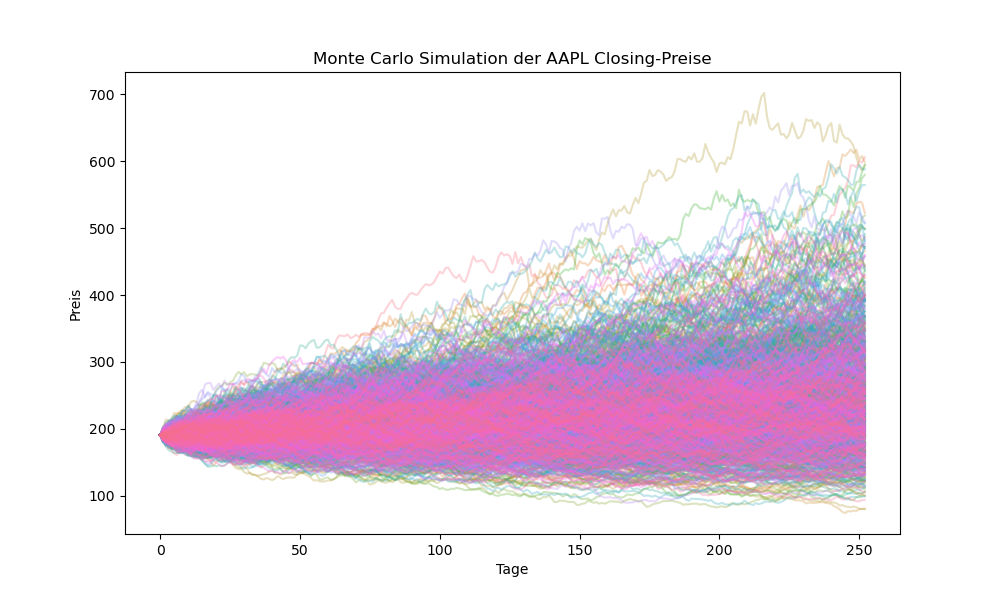
\includegraphics[width=\textwidth]{MonteCarloPlot.png}
        \caption{Monte Carlo Simulation der AAPL-Aktienkurse}
        \label{fig:montecarlo}
    \end{minipage}
    \hfill
    \begin{minipage}{0.48\textwidth}
        \centering
        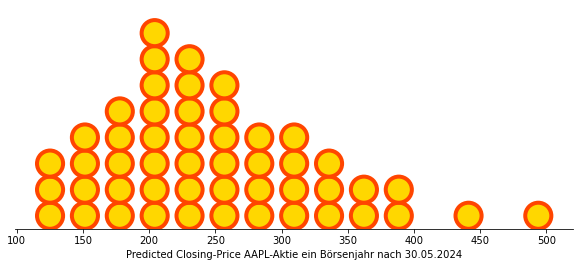
\includegraphics[width=\textwidth]{../Bilder/AAPL_QDP.png}
        \caption{Quantile Dotplot der simulierten AAPL-Aktienkurse}
        \label{fig:quantiledotplot}
    \end{minipage}
    \caption{Gegenüberstellung herkömmliche Visualisierung vs. Quantile Dotplot}
    \label{fig:nebeneinander}
\end{figure}

\subsection{Diskussion}
Die Monte Carlo Simulation ermöglicht eine Analyse der zukünftigen Preisbewegungen der Aktie. Durch die Darstellung als Quantile Dotplot können wir die Unsicherheiten und Risiken, die mit den zukünftigen Preisbewegungen verbunden sind, besser verstehen. Dies hilf Investoren dabei, besser Entscheidung im Bezug auf die Investition in diese Aktie zu treffen.

Vergleicht man in Abbildung \ref{fig:nebeneinander} die Verläufe der einzelnen Simulationen aufgezeichnet im Vergleich zu der Darstellung der Verteilung in einem Quantile Dotplot, ist klar zu erkennen, aus welcher Darstellung man eher die Tendenzen der zukünftigen Kursverläufe erkennen kann. Während der Monte Carlo Plot die Unsicherheiten in den einzelnen simulierten Kursverläufen darstellt, bietet der Quantile Dotplot eine kompaktere und klarere Darstellung der Verteilung der Endpreise. Man beachte, dass dies zum Beispiel als erste schnelle Analyse der Aktie genutz wird, wobei ein Investor etliche dieser am tag sehen würde.
Der Quantile Dotplot bringt einen intuitiveren Überblick und wie bereits ausgearbeitet definitive Vorteile für beide Denkprozesse nach Sektion 2.2.

\section{Fazit und Ausblick}

\subsection{Zusammenfassung der wichtigsten Erkenntnisse}

In dieser Arbeit wurde ntersucht, wie sich die Visualisierung von Unsicherheiten und Risiken auf die Entscheidungsfindung auswirkt. Es wurden verschiedene Theorien zur Entscheidungsfindung unter Unsicherheit betrachtet, darunter die Erwartungsnutzentheorie und die Dual-Process-Theorie. Zudem wurde die Bedeutung der Visualisierung von Unsicherheiten anhand einer Fallstudie im Bereich Fantasy Football untersucht. Es zeigte sich, dass Quantile Dotplots eine effektive Methode zur Darstellung von Unsicherheiten sind und die Entscheidungsfindung verbessern können.

Die Anwendung dieser Erkenntnisse auf die Finanzwelt wurde durch eine Monte Carlo Simulation für eine Aktienprognose demonstriert. Die Visualisierung der Ergebnisse mittels Quantile Dotplots zeigte die Verteilung der möglichen zukünftigen Preise und half, die Unsicherheiten zu quantifizieren.

\subsection{Vorschläge für künftige Forschung}

Da der Forschungsbereich der Unsicherheitsvisualisierung reg ist, aber in der Domäne der Finanzen wenig bis kaum darüber geforscht wird, trotz der vielen Prognosen und Entschidungen welche dort gefällt werden, sind weitreichende Studien zur Wirkung bereits entwickelter Unsicherheitsvisualisierungen aus anderen Domänen in der Finanzwelt mehr als wünschenswert.
Anders als in der Medizin geht es dort nicht darum Entscheidungen zu stützen, welche über Menschenleben entscheiden können, aber dennoch um Existenzen. Auch sollen Laien einfacher die schwere Ihrer Entscheidungen nachvollziehen können.
